\cotefile{69}
\scanpage{50}
\mspage{9}
\unsure{Convention|Convent.|commutant} : $\Delta$ objet de base

\uline{III} \uline{Relations avec} $E_6$

Soit $\Delta$ un graphe cubique

\uline{Définition} On appelle \uline{racines} de $\Delta$ les différences \inserted{$\delta'-\delta$,}
\inserted{dans $\widehat E$,} de sommets distincts non liés de $\Delta\subset\widehat E(\Delta)$

Leur ensemble $R(\Delta)$ est considéré comme partie de $E(\Delta)={}$orthogonal de $\lambda_\Delta$

$R(\Delta)$ est stable par $r\longmapsto-r$.

\deleted{\uline{Théorème} $R(\Delta)$ est un système de racines.}

\deleted{On a $(\delta'-\delta$} Si $r$ est une racine, on a

Avec $r=\delta'-\delta$.
\[
\underline{r^2=\delta'^2+\delta^2=-2}.
\]
Faisons la liste \inserted{explicite dans le cas \unsure{du|de} $\Delta_0$ \inserted{\unsure{Simplexe standart.|graphe standard}}}, --- \unsure{trouve|trouvons} que les différences \inserted{virtuelles}
$\delta'-\delta$ en question sont six à six de la façon suivante en termes de \unsure{suites|sextes|sixtes} \inserted{(``duales'')}
$(\alpha_1,\ldots\alpha_6)(\alpha'_1,\ldots,\alpha'_6)$
\deleted{$\unsure{\zeta_1\ldots\zeta_h=\zeta'_1\ldots\zeta'_h|\xi'_1-\xi_1=\xi'_2-\xi_2=}$} de sommets satisfaisant :
\[
\left\{\begin{aligned}
&\alpha_i\text{ lié à }\alpha'_j\text{ ssi }i\ne j,\quad
  \text{les }\alpha_i\text{ non liés mutuellement,}\\
&\text{les }\alpha'_i\text{ idem, en posant }\quad
 r_\alpha=\alpha'_1-\alpha_1=\alpha'_2-\alpha_2=\dots=\alpha'_6-\alpha_6
\end{aligned}\right.
\]

\deleted{\unsure{$r_0$}}

racines :
\[
\begin{aligned}
1\;&\left\{\begin{aligned}r_0&=2\eta-\textstyle\sum\zeta_i=\lambda-\eta\\
r_0&=\zeta'_{\unsure{1|a}}-\zeta_1=\zeta'_2-\zeta_2=\ldots=\zeta'_6-\zeta_6\end{aligned}\right.
&&\text{déduit de }\left\{\begin{aligned}&(\zeta_1\ldots,\zeta_6)\\&(\zeta'_1,\ldots\zeta'_{\unsure{0|6}})\end{aligned}\right.\\[4pt]
15\;&\left\{\begin{aligned}&r_{ij}=\zeta_i-\zeta_j\\&1\le i<j\le6\end{aligned}\right.
&&\text{déduits de }\left\{\begin{aligned}
&(\zeta_j,\zeta'_j,(\zeta_{i\unsure{h|k}})_{h\ne i,j},\deleted{\unsure{\zeta_{ij}}})\deleted{\unsure{\zeta'_6})}\\
&(\zeta_i,\zeta'_i,(\zeta_{jh})_{h\ne i,j})\end{aligned}\right.\\[4pt]
20\;&\left\{\begin{aligned}&r_{ijh}=\eta-\zeta_i-\zeta_j-\zeta_h\\&1\le i<j<h\le6\end{aligned}\right.
&&\text{déduits de }\left\{\begin{aligned}
&(\zeta_i,\zeta_j,\zeta_h,\zeta_{\ell m},\zeta_{mn},\zeta_{n\ell})\\
&(\zeta_{jh},\zeta_{hi},\zeta_{ij},\zeta'_n,\zeta'_\ell,\zeta'_m)\end{aligned}\right.
\end{aligned}
\]
avec \deleted{$1\le\ell<m<n\le6$} \inserted{$\ell,m,n$} les trois él\textsuperscript{ts} de $[1,6]$ distincts de $i,j,h$ (ou selon cas \unsure{prec.|p.ex.}).

et les \deleted{\unsure{différentielles|opposées}} obtenus en échangeant $\alpha$ et $\alpha'$
% archive sheet number: 49

\scanpage{51}
\mspage{10}
Cela fait $72=2\times36$ racines, associées aux $27\times16=6\times72$
\inserted{$=432$} couples $(\delta',\delta)$ de sommets distincts non liés

On vérifie de plus que pour \unsure{tte|les|tt} \unsure{racine|racines} $r_\alpha$, associé à un système
$\left\{\begin{aligned}\alpha&=(\alpha_1,\ldots,\alpha_6)\\\alpha'&=(\alpha'_1,\ldots,\alpha'_6)\end{aligned}\right.$, on a
\[
r_\alpha\alpha_i=(\alpha'_i-\alpha_i)\alpha_i=0-(-1)=1,\quad
\inserted{\text{de }=}\ r_\alpha(\alpha'_i)=-1
\]
\[
\left\{\begin{aligned}
r_\alpha\cdot\alpha_i&=1\\
r_\alpha\,\alpha'_j&=-1\\
r_\alpha\,\deleted{\unsure{\alpha_j}}\delta&=0\quad\text{si }\delta\in\Delta_0\text{ distinct de }\alpha_i,\alpha'_i .
\end{aligned}\right.
\]
% slanted
\margin{ceci provient du fait que $\unsure{\exists}$ \unsure{couple} \deleted{\unsure{$(\alpha_i,\alpha'_i)$|$(\alpha'_i,\alpha_i)$}} (\unsure{en} \deleted{\unsure{fait}} \unsure{il y en a ex. $4$|il y en a $4$}) tel que $\delta$ soit \unsure{lié} à $\alpha_i,\alpha'_i$ i.e. $\delta$ orthog. à $\alpha_i,\alpha'_i$ donc à leur diff. $r$}

Donc cela explicite \inserted{(pour un $\Delta$ cubique génér. ?)} comment à une racine $r$ sont associées deux parties $\alpha(r),\alpha'(r)$ de $\Delta$ : l'une des $s$ \inserted{$\in\Delta$} tels que $rs=1$ resp. $-1$ ; On trouve une corr. $1$-$1$ entre ces parties \inserted{$\alpha$} et les \deleted{parties} racines, le passage de $r$ à $-r$ revenant à échanger $\alpha$ avec le $\alpha'$ dual \ldots

Bien entendu, \deleted{les} \inserted{les} parties basiques de $\Delta$ \unsure{sont} associées à \deleted{des} \inserted{une} racine. Pour voir que l'inverse est vrai, il suffit de vérifier que les parties écrites ci-dessus \inserted{dans le cas standard} sont basiques (et ils sont groupés alors par couples de bases duales).

\deleted{Il reste \unsure{sont} \unsure{donc} que :} \deleted{\inserted{à vérifier que} dans $\widehat E(\Delta_0)$}
\[
\deleted{\alpha'_i-\alpha_i=r\quad \text{indépendant de }i, \quad\text{considérons}}
\]
\[
\begin{aligned}
&\deleted{\eta(\alpha)=\lambda-r(\alpha)=\lambda-r}\\
&\deleted{\text{et }\textstyle\sum\alpha_i=r+\zeta(\alpha)\ ;\quad\text{vérifions qu'il est \unsure{divisible|accessible} par 2 dans}}\\
&\deleted{\widehat E,\qquad\underbrace{\textstyle\sum\alpha_i}_{\zeta(\alpha)}\quad
 \text{sont }\eta(\alpha)=\tfrac12(r+\zeta(\alpha))}
\end{aligned}
\]
\deleted{On trouve dans les cas \uline{listés}}
\[
\left\{\begin{aligned}
&\deleted{\eta(r_0)=\eta(\zeta_1,\ldots\zeta_6)=\eta}\\
&\deleted{\eta(-r_0)=\eta(\zeta'_1\ldots\zeta'_6)=\eta'=5\eta-2\zeta=5\eta-2\textstyle\sum\zeta_i}\\
&\deleted{\eta(\zeta_i-\zeta_j)=\eta(\zeta_j,\zeta'_j,(\unsure{\zeta_{ih}|\xi_{ik}}))=3\eta-2\zeta_i-\textstyle\sum_{h\ne i,j}\zeta_h=(=\lambda)-\zeta_i+\zeta_j=\lambda-r.}
\end{aligned}\right.
\]
\[
\begin{aligned}
&\deleted{\eta(\alpha)}\quad\deleted{r=2\eta(\alpha)-\underbrace{\textstyle\sum\alpha_i}_{\zeta(\alpha)}\quad\text{i.e. que}}\\
&\deleted{\underset{\scriptscriptstyle\sum\alpha_i}{\underset{\scriptscriptstyle\Vert}{\zeta(\alpha)}}=2(\lambda-r)-r=2\lambda-3r}
\end{aligned}
\]
% archive sheet number: 50

\scanpage{52}
\mspage{11}
(il y a \unsure{princip\textsuperscript{lt}|principalement|manifestement} \unsure{2 cas|le cas|4 cas} à distinguer, ceux des $r=r_{ij}$ et $r=r_{ijh}$ \ldots) dans le cas standard,
\[
\alpha=\alpha^{ij}=(\zeta_i,\zeta'_j,(\unsure{b'_{ih}|\zeta'_{ih}|\xi_{ik}})_{h\ne i,j})\quad\text{et}\quad
\alpha=\alpha^{i,j,h}=(\zeta_i,\zeta_j,\zeta_h,\zeta_{\ell m},\zeta_{mn},\zeta_{\unsure{np|n\ell}})
\]
sont des bases. \deleted{\unsure{si|i.e.}} \inserted{Soit} \deleted{si} \deleted{$\alpha=(\alpha_1,\ldots\alpha_6)$} $\alpha'=\{\alpha'_1,\ldots,\alpha'_6\}$,

\deleted{$\Rightarrow\ \forall\ 1\le i<j\le6,\ \exists!\ \unsure{\delta}\in\alpha_{ij}\in\Delta$ lié à \unsure{$\zeta_i$} $\alpha_i,\alpha'_j$}

Si $1\le i<j\le6$, \deleted{$\unsure{\delta}$}$\alpha_i$ et $\alpha'_j$ sont liés, donc $\exists!\ \delta\in\Delta_0$ lié à $\alpha_i$ et $\alpha'_j$, soit $\alpha_{ij}$. \deleted{Les $\alpha_{ij}$} Tout $\delta\in\Delta_0$ distinct des $\alpha_i,\alpha'_i$ est-il de la forme $\alpha_{ij}$ i.e. est-il lié à un des $\alpha_i$ et à un des $\alpha'_j$ ? \deleted{S'il n'était lié à aucun des \ldots}

\deleted{Vérifications fastidieuses \ldots} Meilleur procédé :

Comme pour tte racine $r$ on a $rr=-2$, l'endomorphisme (``symétrie \unsure{parr à|par à|par} $r$'')
\[
s_r\deleted{\unsure{(|:}}x\longmapsto x+(x.r)r\qquad\widehat E\longrightarrow\widehat E
\]
[dont l'ens des p\textsuperscript{ts} fixes est $r^\perp$, et qui transforme $r$ en $-r$] est un autom de \deleted{orthogonal} \inserted{$(\widehat E,\widehat\varphi\ \text{forme fond.})$} qui évidemment respecte aussi $\lambda$ (car $r\in E=\lambda^\perp$). Montrons qu'elle applique $\Delta$ dans $\Delta$. [Il suffit de regarder le cas standard, et de regarder alors les trois cas $r=r_0$, $r=r_{ij}$, $r=r_{ijh}$.]

\deleted{\unsure{$r_0$}} Notons d'abord, de façon générale, que si $r$ est associé à $(\alpha_1,\ldots\alpha_6),(\alpha'_1,\ldots\alpha'_6)$ ($r=\alpha'_i-\alpha_i$ pour $1\le i\le\unsure{r|6}$) on a
\[
\boxed{s_r\alpha_i=\alpha'_i,\quad s_r\alpha'_i=\alpha_i}
\]
Car $\left\{\begin{aligned}r.\alpha_i&=1,\ r\alpha'_i=-1\end{aligned}\right.$

\deleted{Il reste} à voir l'effet de $r$ sur les autres éléments de $\Delta$ --- et de montrer que
\[
\boxed{s_r\delta=\delta\quad\text{si }\delta\notin\{(\alpha_i),(\alpha'_i)\}}
\]
% archive sheet number: 51

\scanpage{53}
\mspage{12}
\unsure{relation déjà notée|résultat déjà noté|relations déjà notées} plus haut

\deleted{a) Cas de $r_0$ --- Il provient des relat\textsuperscript{ons} \unsure{$r$}}

\deleted{$s_{r_0}(\unsure{\zeta_{ij}|\xi'_j})=$}

Soit $W$ le groupe d'autom de $(\widehat E,\widehat\varphi,\lambda)$ \inserted{(\unsure{le même|le mien|ou ce qui revient au même} de $\Delta$)} engendré par les $s_r$. Je dis que $W$ \uline{opère transitivement sur l'ens des racines}, donc aussi sur l'ens des parties \inserted{$(\subset\mathfrak P_6(\Delta))$} de $\Delta$ associées --- qui sont donc toutes des parties basiques. Pour ceci, notons d'abord que
\[
\begin{aligned}
&\deleted{s_{r_{ij}}\,\zeta'_k=\left\{\zeta_k\quad k\ne i,j\right.}\\
&s_{r_{ij}}\text{ est l'autom de }\Delta_0\ \deleted{\text{engendré par}}\ \inserted{\text{associé à}}\ \text{l'élém}^{\rm t}\\
&\qquad\text{de }\unsure{\mathfrak S|\mathscr S}_6,\quad\deleted{\text{permutation}}\ \inserted{\deleted{\text{une}}\ \text{transposition}}\ \text{de }i\text{ et }j.
\end{aligned}
\]
(vérification immédiate) donc

\uline{Corollaire} $W$ contient $\mathfrak S_6$

\uline{Corollaire} les $r_{ij}$ sont conjugués par $W$, et les $r_{ijh}$ sont conjugués par $W$.

Il reste donc à voir que $r$ est conjugué à un $r_{ij}$ et à un $r_{ijh}$. \deleted{Car} Or on vérifie \deleted{\unsure{$r_\Delta$}} de suite
\[
s_{r_{ijh}}(r)=r_{\ell,m,n}
\]
donc $r$ conjugué aux $\unsure{r_{\ell mn}|r_{\ell,m,n}}$, et
\[
s_{r_{ijh}}(r_{i\unsure{\ell|g}})=r_{jh\ell}
\]
donc \deleted{\unsure{donc} $r_{i\ell}$ \unsure{est}} un des $r_{\ldotp\ldotp}$ ($r_{i\ell}$) conjugué à un des $r_{\ldotp\ldotp\ldotp}$ ($r_{jh\ell}$) et on a gagné.

On sait donc plus précisément, compte tenu que $W\supset\mathfrak S_6$

\uline{Corollaire} $W$ est transitif sur l'ens des \deleted{bases} racines, sur l'ens des bases \inserted{(qui sont en corr. $1$-$1$ avec les racines)}, sur l'ens des bases \uline{ordonnées}, et sur $V$ ens \deleted{des} des couples $(\delta',\delta)$ de deux sommets non liés. Enfin, $W$ est identique au groupe de tous les automorphismes de $\Delta$.
% archive sheet number: 52

\scanpage{54}
\mspage{13}
\deleted{\unsure{Prouvons|Prenons|Proposition}.}

\uline{Corollaire}\quad $\operatorname{Card} W=72\mathbin.6!=2^7\mathbin.3^4\mathbin.5$

En effet, $W$ est \uline{simplement} \uline{transitif} sur $V$ ens des bases ordonnées, qui \unsure{sont au nb|est au nb|a un card} de $72\mathbin.6!$. (car il y a $72$ parties basiques i.e. $72$ racines \ldots)

\uline{Th}\quad $(E(\Delta),R(\Delta))$ est un \deleted{\unsure{ens de|un}} \inserted{système de} racines de type $E_6$, \inserted{et $E(\Delta)$ engendré par $R$.} et si $(\zeta_1,\ldots\zeta_6)$ est une base ordonnée de $\Delta$, le système de racines
\[
\begin{aligned}
&\deleted{\alpha_1=\zeta_1\unsure{-}\zeta_2}\\
&\deleted{\unsure{\alpha}}r_1=r_{12}=\zeta_1-\zeta_2\\
&\deleted{\unsure{\alpha}}r_2=r_{23}=\zeta_2-\zeta_3\\
&\ldots\\
&r_{\deleted{6}5}=r_{56}=\zeta_5-\zeta_6\\
&r_6=r_{123}=\deleted{\unsure{2\eta-\zeta=2\eta-\textstyle\sum\zeta_i}}\ \eta-\zeta_1-\zeta_2-\zeta_3
\end{aligned}
\]
est un système de racines simples, suivant le diagramme
\diagram{\begin{tikzcd}[ampersand replacement=\&,column sep=1.1em,row sep=.65em]
\overset{r_1}{\bullet}\arrow[r,dash]\&\overset{r_2}{\bullet}\arrow[r,dash]\&\overset{r_3}{\bullet}\arrow[r,dash]\arrow[d,dash]\&\overset{r_4}{\bullet}\arrow[r,dash]\&\overset{r_5}{\bullet}\\
\&\&\underset{r_6}{\bullet}
\end{tikzcd}}

\inserted{Pour $r\in R$,} La symétrie $s_r$ restreinte à \inserted{$E={}$}$E(\Delta)$ est la sym. associée au syst. de racines et à $r$, et $W$ (identifié à un groupe d'autom de $E$) est \inserted{donc} le groupe de Weyl du syst. de racines. La forme bil. \inserted{sym.} $\varphi=\overline\varphi\mid E$ est caractérisée par la propriété d'être invariante \inserted{par $W$} et de satisfaire $r.r=-2$ $\forall r\in R$.
% archive sheet number: 53

\scanpage{55}
\mspage{14}
\uline{Dém} \deleted{Tout ceci}

$E$ est engendré par $R$, et même par $r_1\ r_2\ r_3\ r_4\ r_5\ r_6$

Car des sommes partielles des $r_i$ \inserted{$1\le i\le5$} donnent les $\zeta_{i}-\zeta_j$ $(i<j)$, et il est clair que les $\zeta_i-\zeta_1$ $(1\le i\le6)$ et \deleted{$\unsure{\eta-\lambda-2\zeta_1|\eta-2\lambda}=\eta-\lambda$ (car $\lambda-\eta=r_0=r'_6$} \inserted{$\eta-3\zeta_1$} engendrent $E$ $(=\operatorname{Ker}(\widehat E\xrightarrow{\lambda\, .}\mathbb Z))$ puisque \deleted{$\lambda.\zeta_1=1$, et} $\lambda.\zeta_i=1,\ \lambda.\eta=3$. Donc $E$ engendré
\deleted{$\eta,\zeta_1,\ldots,\zeta_6$ engendrent $\widehat E$ et leurs produits avec $\lambda$ sont $3\ 1$}
par \inserted{les} $\zeta_1-\zeta_i$ et \deleted{$\eta-3\zeta_1=3\zeta_1-\eta$} \inserted{$\eta-3\zeta_1$}
\deleted{\unsure{$= \lambda+\eta$|$3\lambda-\eta$}} donc par $r_1\ldots r_5$ et $\eta-3\zeta_1$. Reste à prouver que $\eta-3\zeta_1$ est une comb. des $r_i$, \unsure{rappeler|rappelons}
\[
\begin{aligned}
r_6&=\deleted{\unsure{r_0=2\eta}}\ \eta-\zeta_1-\zeta_2-\zeta_3,\\
&=(\eta-3\zeta_1)+(\zeta_1-\zeta_2)+
\underset{\substack{\Vert\\(\zeta_1-\zeta_2)+(\zeta_2-\zeta_3)}}{(\zeta_1-\zeta_3)},\quad\text{\unsure{gagné|on gagne}.}
\end{aligned}
\]

On sait déjà que les $s_r$ transforment $\Delta$ en lui $=$, donc $R$ en lui-$=$, et comme $s_r$\deleted{\unsure{$=(r\mapsto-r)$}} \inserted{$=(x\longmapsto x+r^\star(x)r)$ avec $r^\star(r)=-2$,} on conclut que $R$ est un syst. de racines --- compte tenu que deux racines distinctes \unsure{non opp.} sont \inserted{non} proportionelles. \deleted{Que} \inserted{Prouvons que} $\alpha_1\ldots\alpha_6$ sont un syst. de racines simples. \deleted{\unsure{on voit en}}

On a déjà vu
\[
\boxed{r_{ij}=r_i+r_{i+1}\ldots+r_{j-1}\qquad\text{si }i<j}
\quad\text{(\unsure{pr $i$ ou|pris en|pour $1\le i,$} }j=\unsure{5|i},\quad\text{\unsure{max.|max|$\le$} : }5\text{)}
\]
On a
\[
\begin{aligned}
r_{ijh}&=\eta-\zeta_i-\zeta_j-\zeta_h=(\eta-\zeta_1-\zeta_2-\zeta_3)
+\underbrace{(\zeta_1-\zeta_i)}_{r_{1i}}+\underbrace{(\zeta_2-\zeta_j)}_{r_{2j}}+\underbrace{(\zeta_3-\zeta_h)}_{r_{3h}}\\
&=\deleted{\unsure{\Sigma_6+}}\ r_{123}+r_{1i}+r_{2j}+r_{\unsure{2|3}h}
\end{aligned}
\]
donc
\[
r_{ijh}=r_6+(r_1\ldots+r_{i-1})+(r_2\ldots+r_{j-1})+(r_3+\ldots r_{h-1})
\]
% archive sheet number: 54

\scanpage{56}
\mspage{15}
i.e.
\[
\boxed{r_{ijh}=r_6+\deleted{\unsure{1}}(r_1+\ldots+r_{i-1})+\deleted{\unsure{1}}(r_2\ldots+r_{j-1})
\deleted{\unsure{{}+2r_1+1r_2|2r_1+r_2}}+(r_3\ldots+r_{h-1})}
\]
pour $i<j<h$
\[
\left(\begin{aligned}\text{poids }&i+j+h-5\\\text{maximum }&10\end{aligned}\right)
\quad
\deleted{\begin{gathered}\text{poids }1+3(i-1)+2(j-i\unsure{{}+1|{}-1})+h-j\unsure{{}+1}\\
=1+(i+j+h\unsure{{}-5})=i+j+h-5\\\text{max. }10\end{gathered}}
\]
enfin
\[
\begin{aligned}
r_0&=2\eta-\textstyle\sum\zeta_i=(\eta-\zeta_1-\zeta_2-\zeta_3)+(\eta-\zeta_4-\zeta_5-\zeta_6)\\
\text{i.e.}\quad &=\underbrace{r_{123}}_{\deleted{\unsure{r_0+2r_1+r_2|r_6+2r_1+r_2}}}+r_{456}
\end{aligned}
\]
donc
\[
\boxed{r_0=\deleted{\unsure{r_6+2r_1}}\ r_1+2r_2+3r_3+2r_4+r_5+2r_6}
\qquad(\text{poids }\deleted{\unsure{14}}11)
\]
(NB On a là la ``plus grande racine'' \deleted{\unsure{évidt}}).

Donc tte racine est \deleted{somme} comb. lin. à coeff. entiers tous de $=$ signe de $r_1\ldots r_6$, qui forment donc un syst. de racines simples. Enfin, on vérifie immédiatement que $r_i.r_j=0$ \inserted{pour $i<j$} sauf dans les cas \deleted{$j\ne6$} $j=i+1\deleted{\unsure{{}\ne}} \le5$ et \unsure{le p.|les p.|le cas} $j=6,\ i=3$, ce qui montre que le diagramme est $E_6$. ---

\uline{Corollaire} Soit $\widetilde W$ le groupe des autom du syst. de racines $(E(\Delta),R(\Delta))$, et considérons l'application canonique
\[
W=\operatorname{Aut}(\Delta)\lhook\joinrel\longrightarrow\widetilde W
\]
Alors \unsure{la} l'image est d'indice $2$ dans $\widetilde W$.

En effet, on sait que $\widetilde W/W\simeq$ groupe des autom. du diagramme de Dynkin, qui est ici d'ordre $2$.
% archive sheet number: 55
% archive sheet number: 56 (at the far right of the facing-page edge)

\scanpage{57}
\mspage{16}
Donc la donnée de $\Delta$ est un peu plus fine que celle du syst. de racines associé de type $E_6$ (et a fortiori que la donnée d'une forme \unsure{bilinque|bilinéaire|bil. sym.} \inserted{non dég.} sur un $\mathbb Z$-Module $E$ \ldots). On peut interpréter cette donnée suppl. comme la donnée, \deleted{\unsure{pour un syst}} d'un des deux sommets
\diagram{\begin{tikzcd}[ampersand replacement=\&,column sep=small,row sep=tiny]
\alpha\,\bullet\arrow[r,dash]\&\bullet\arrow[r,dash]\&\bullet\arrow[r,dash]\arrow[d,dash]\&\bullet\arrow[r,dash]\&\bullet\,\beta\\
\&\&\bullet
\end{tikzcd}}
$(\alpha,\beta)$ (extrémités longues) ``\uline{du}'' diagramme de Dynkin de $(E,R)$ (i.e. d'un des syst. simples de racines). Mais on aimerait expliciter, en termes de la géométrie interne à \deleted{\unsure{$R$},} un syst. de racines $(E,R)$ de type $E_6$, comment \deleted{\unsure{exactement à}} \inserted{ce supplément} de structure permet de récupérer le graphe cubique $\Delta$.

Définissons
\diagram{\begin{tikzcd}[ampersand replacement=\&]\Delta\arrow[r,"i"]\&E\end{tikzcd}}
par
\[
i(\delta)=3\delta-\lambda\qquad(\in E\text{ car }\delta.\lambda=1,\ \lambda.\lambda=3)
\]
de sorte que \unsure{pr|pour}
\[
\deleted{\unsure{i\delta|i(\delta)}}\ i(\delta)i(\delta')=9\delta.\delta'-6+3=9\delta\delta'-3
\]
donc
\[
\left\{\begin{aligned}
i(\delta)^2&=-12\\
i(\delta)i(\delta')&=\begin{cases}9&\text{si }\delta,\delta'\text{ liés}\\-3&\text{si }\delta\ne\delta'\text{ non liés}.\end{cases}
\end{aligned}\right.
\]
Donc $i$ est une bijection de $\Delta$ dans \inserted{une partie $\Delta'$ de} l'ens $\unsure{\mathscr E|\mathfrak E}_{(12)}$ des éléments \inserted{$x$} de $E$ satisfaisant
\[
x.x\unsure{{}^{\scriptscriptstyle\leftarrow}}=-12
\]
et sur l'image $\Delta'$ de $\Delta$, \deleted{\unsure{On}} relation ``lié'' s'exprime par
\[
x,x'\text{ liés}\Longleftrightarrow x.x'=9
\]
Bien entendu, $W$ invarie $\Delta'$. \deleted{\unsure{Et}} D'ailleurs $R$ est déduit de $\Delta'$ \deleted{comme} par la Condition que \unsure{!|?}
% archive sheet number: 56

\scanpage{58}
\mspage{17}
\[
3R=\{\deleted{\unsure{\text{avec}}}\deleted{\unsure{\varnothing}}\ x'-x\mid x,x'\in\Delta'\}.
\]
Mais \deleted{soit $\widetilde\Delta$ notons que $\widetilde\Delta'$} notons que
\[
-\Delta'=\{-(3\delta\deleted{\unsure{+}}-\lambda)=\lambda-3\delta\mid\delta\in\Delta\}
\]
est aussi invariant par $W$ et contenu dans $S_{-12}$, d'ailleurs \deleted{\unsure{tel}} $\Delta'\cap(-\Delta')=\varnothing$ car $3\delta-\lambda=\lambda-3\delta'$ implique $3(\delta+\delta')=2\lambda=2(3\eta-\zeta)$ or $2\lambda=6\eta-2\zeta$ n'est pas divisible par $3$ dans $\widehat E$ !

\deleted{Notons que $W$} \unsure{Ceci|Cela} montre que $-\operatorname{id}_E\notin W$, et comme c'est $\in\widetilde W$, on trouve
\[
\widetilde W=W\times\underbrace{\mathbb Z/2\mathbb Z}_{\substack{\text{engendré par}\\\operatorname{id}_E}}
\]
\deleted{\unsure{$\Delta$}} La réunion $\widetilde\Delta^{\unsure{+|=}}=\Delta'\cup(-\Delta')$ est donc \deleted{\unsure{intrinsèqut|intrinsèque}} \inserted{canoniqt} associé au syst. de racines (indépendamment de son obtention par un $\Delta$) et il se décompose en deux orbites sous $W$. Le choix d'une orbite équivaut au choix du syst. de racines. On aimerait l'expliciter, \inserted{ainsi que $\widetilde\Delta$,} via la géométrie interne du syst. de racines.
% archive sheet number: 57

\scanpage{59}
\uline{Graphes cubiques}

Un graphe $\Delta$ est dit \inserted{\uline{graphe}} \uline{cubique} si \deleted{\unsure{les arêtes}} ses arêtes sont déterminées par leurs extrémités, (qui sont distinctes, et s'il existe \deleted{deux} parties $I$, \inserted{$I'$,} de l'ens des sommets satisfaisant les conditions suivantes

a) \deleted{\unsure{$I$ de}} $\operatorname{card} I=\operatorname{card} I'=6$, $I$ et $I'$ disjoints

b) $\forall i\in I,\ \exists!\ i'\in I'$ tel que $i'$ non lié à $I$, et $\forall i'\in I',\ \exists!\ i\in I$ tel que $i$ non lié à $I$ [donc $I$ et $I'$ sont en corr. biunivoque par la relation ``$i$ n. lié à $i'$'' \deleted{\unsure{k}}, soit $\unsure{i|\iota}:\deleted{\unsure{I\to I'}}\ I\cup I'\longrightarrow I\cup I'$] \deleted{\unsure{tel}}

c) $\forall$ partie $J$ \inserted{$=\{i,j\}$} à deux éléments de $I$, $\exists!\ \zeta_J=\zeta_{ij}\in\Delta$ \inserted{$-J\cup i(J)$} qui soit lié aux \unsure{4|a|\deleted{deux}} éléments \deleted{$i,j$ et} de $J\cup i.(J)$, et non lié aux autres éléments de $I\cup I'$.

\deleted{[\unsure{donc c'est donc que} $\lambda_J\notin I\cup I'$}

[Il est clair que $J\longmapsto\lambda_J$ est une appl. \uline{injective} de $\mathfrak P_2(I)$ dans $\Delta-(I\cup I')$

d) L'application précédente
\[
\mathfrak P_2(I)\longrightarrow\Delta-(I\cup I')
\]
est \deleted{bijective} surjective (donc bijective), i.e. $\forall\lambda\in\Delta-I\cup I'$, \deleted{$\exists J\in\mathfrak P_2(\Delta)$ telle que $\lambda$ soit lié à $J\cup i(J)$,} l'ens. des éléments de $I\cup I'$ auxquels $\lambda$ est lié est de cardinal $4$ et stable par $i$.

e) Si $J,J'\in\mathfrak P_2(I)$, $J\ne J'$, alors $\zeta_J$ et $\zeta_{J'}$ sont liés ssi $J\cap J'=\varnothing$.

\centerline{---}

Graphe cubique $\Delta(I)$ défini par ens $I$ de card. $6$.

$\Delta$ cubique ssi $\Delta\simeq\Delta(I)$ (pour un $I$ de card. $6$, ou pour tous)
% archive sheet number: 58

\scanpage{60}
Pour tt $i\in I$, $\unsure{i|\iota}(i)=i'$ est l'unique élément \uline{de $\Delta$} tel que $i'$ soit lié à \uline{tous les} él. de $I-\{i\}$. Donc la connaissance de $I$ implique déjà celle de $I'$. On appelle $I$ \uline{partie basique}. Si $I$ est telle, $I'$ est une partie basique, dite \uline{partie basique associée}. Base (ou partie basique ordonnée).

\deleted{\uline{\unsure{Prop}} La cat. des graphes cubiques}

Bibase : \deleted{bibase ordonnée \unsure{est un}} \inserted{él. de} $\mathfrak P_2(\mathfrak P_6(\Delta))$ formé de deux \deleted{\unsure{b}} bases associées.

\uline{Prop} a) La cat. \inserted{(pour les isos)} des graphes cubiques munis d'une base (resp. base ordonnée) est équivalente \inserted{can\textsuperscript{t}} à la cat. $\mathrm{Ens}_6$ des ens. à $6$ él (avec iso.) (resp. à la cat. ponctuelle)

b) La catégorie des gr. cub munis d'une bibase (resp. bibase ordonnée) est \inserted{can} équivalente à la catégorie \inserted{$(\mathrm{Ens}_6)\times(\mathrm{Ens}_2)$} des couples $(E,b)$ d'un ens. à six él. et d'un ens à $2$ él.

c) Soit $\Delta$ graphe cubique. L'ens des bases ordonnées de $\Delta$ est can. isom à
\[
\operatorname{Isom}_{\rm gr}(\overbrace{\Delta([1,6])}^{\Delta_0},\Delta),
\]
donc est un torseur à droite sous $W_0=\operatorname{Aut}\Delta_0\deleted{([1,6])}$, à gauche sous $W=\operatorname{Aut}(\Delta)$.

\uline{Th} Considérons $\Delta=\deleted{\Delta_0={}}\Delta(\unsure{\mathrm{II}|\mathbb I|I})\deleted{\unsure{\in\mathfrak P}}$, \deleted{\unsure{alors|Alors}} \inserted{les él. de $I$ dans $\Delta$ sont notés $\zeta_i$} avec sa base canonique \deleted{\unsure{ln}} $I$ et la base associée $I'$.

Les bases de $\Delta$ sont les parties \inserted{obtenues de la façon} suivantes.
% slanted
\margin{énoncer plutôt en termes de bibases \ldots}

(i) $I$ et $I'$ \deleted{\unsure{:}} (soit $2$ parties)

(ii) $\forall\ \deleted{\unsure{p\in\mathfrak P_2(\Delta)|J\in\mathfrak P_2(I)}}\ (i,j)\in I\times I-\operatorname{diag}$, $B^{ij}$ désigne la partie de $\Delta$ formée de $\{\zeta_j,\zeta'_j,(\zeta_{ik})_{k\in I-i-j}\}$ (soit $30$ parties)

(iii) $\forall K\in\mathfrak P_3(I)$, $B^{\deleted{\unsure{J}}K}$ désigne la partie \inserted{de $\Delta$} formée des $\{\zeta_i\ (i\in K),\ \deleted{\unsure{\cap}}\ \zeta_J\ (J\in\mathfrak P_2(I-K)\unsure{-|=}\mathfrak P_2(I))\}$ $(20)$

(iv) $\forall K\in\mathfrak P_3(I)$, $B'{}^K$ désigne la partie de $\Delta$
% archive sheet number: 59

\scanpage{61}
formée des $\{\zeta'_i\ (i\in I-K),\ \zeta_J\ (J\in\mathfrak P_2(K)\subset\mathfrak P_2(I))\}$.

La base \deleted{\unsure{associée à|associée}} à $B^{ij}$ est $B^{ji}$, \deleted{de} \inserted{celle ass.} à $B^K$ est $B'{}^K$.

\uline{Corollaire 1}\quad $\operatorname{Card}(\operatorname{Bases}(\Delta))=72$ \inserted{$=8.9=2^3 3^2$}, \deleted{$\operatorname{Card}\operatorname{Aut}(\Delta)=72\mathbin.$}
\[
\operatorname{Card}\underset{\substack{\Vert\\\operatorname{Aut}(\Delta)}}{W}=72.6!=2^7 3^{\unsure{4}}5
\]

\uline{Corollaire 2} $W$ est transitif sur $\Delta$ (ens des sommets), et \deleted{\unsure{sur}} sur l'ens des couples de sommets \inserted{distincts} \inserted{non} liés. Si $(\delta,\delta')$ est un couple de sommets distincts non liés, $\exists!$ base $I$ telle que $\delta\in I$ \deleted{\unsure{et|\&}}, $\delta'\in I'$ base associée (donc $\delta$ et $\delta'$ se correspondent par la bijection can $I\simeq I'$)

\uline{Corollaire 2} La cat. des complexes cubiques $\Delta$ munie d'un él $J\in\mathfrak P_2(\Delta)$ formé de $2$ sommets non liés, est équivalente à la cat. des couples formés d'un ens à cinq éléments et d'un autre à deux él. (\unsure{ce dernier étant|ce dernier est|ces derniers étant} $J$).

\deleted{\unsure{partie particulière|partie liée de cardinal}}

\deleted{Notion de $i$-base, \inserted{(de partie libre de card. $i$)} ($1\le i\le6$) :}

\deleted{\uline{Prop}. \unsure{Pour} \inserted{les} \unsure{bibases} \unsure{parties} libres \inserted{\unsure{ordonnées|ordonnée}} à $3$ él, \unsure{bibases} \unsure{deux} à deux \unsure{qui ne sont liés|non liés|opérées par $W$}. Pour les telles $J$, l'ens $K$ des éléments \inserted{de $\Delta-J$} de \unsure{$\Delta$|$\widetilde\Delta$} liés à tt él de $J$ est de cardinal $6$, et $\exists!$ bibase $\{I'\cup I''\}\simeq I\times\varepsilon$ telle que $J\subset I'\cup I''$, \unsure{stable} \illegible{2} \inserted{et dans} \unsure{le|$K$} \illegible{1} \unsure{les} $2$ él $K=\{K',K''\}$,}

% slanted
\margin{\deleted{et alors $J$ est \deleted{et $*K$} $\unsure{j'j|i'j}$ \unsure{au|ou} $j\in I_1=K/\unsure{i|2}$}}
\deleted{L'ens \inserted{$J'$} des élémts de $\Delta$ liés \unsure{et} \illegible{1} à aucun \unsure{point} de $J$ est de cardinal $3$ \unsure{et tt} él de $K$ est non lié à exactemt $1$ élément de \deleted{\unsure{$J$}} $J'$, d'où une application $K\longrightarrow\deleted{\unsure{\alpha}}J'$. Si la bibase est associée à l'ens à $2$ él. $\varepsilon$, on a donc $K\longrightarrow J'\times\varepsilon$ (ou $K\longrightarrow I'\cup I''\longrightarrow\varepsilon$) qui est un iso.}
% slanted
\margin{\deleted{\uline{NB} la relation entre $J$ et $J'$ est symétrique}}
% archive sheet number: 60

\scanpage{62}
\diagram{\resizebox{\linewidth}{!}{$\begin{array}{r|l|l|l|l|l}
 &\substack{\text{Cat :}\\\Delta\text{ munis de}}&\text{équivalente à}&\text{groupe d'autom}&\substack{\text{Cardinal de l'ens des}\\\text{él. de structure}\\\text{du type envis. de }\Delta}&\\ \hline
1^\circ & \substack{\text{1-base}\\ \bullet \qquad /\!/\!/} & \substack{\deleted{\unsure{\text{structure de}}}\ \deleted{\unsure{\text{torseur}}}\\\text{ens }J\text{ de card}\\5,\ \text{et torseur}\\\text{sous }\mathbb F_2(J)'} & \substack{W_{\mathrm{SO}(10)}\quad\text{ext.}\\\text{de }\unsure{\mathfrak S|\mathscr S}_5\text{ par }(\mathbb Z/2\mathbb Z)^4\\\text{de cardinal}\\2^4 5!=2^7.3.5=1920} & 3^3=27 & 1,10,16\\ \hline
2^\circ & \substack{\text{2-base}\\\bullet\ \bullet} & \mathrm{Ens}_5\times\mathrm{Ens}_2 & \substack{\mathfrak S_5\times\mathfrak S_2\\\text{de card }2.5!=2^4.3.5\\=240} & 2^3 3^3=27.8=216 & 2,5,10,10\\ \hline
3^\circ & \substack{\text{2 base ordonnée}\\\overset{1}{\bullet}\ \overset{2}{\bullet}} & \mathrm{Ens}_5 & \substack{\mathfrak S_5\text{ de card}\\5!=120} & \substack{2^4 3^3=27.16=432\\=6.72} & 1,1,5,5,5,10\\ \hline
4^\circ & \substack{\text{3 base}\\\bullet\ \bullet\ \bullet} & \mathrm{Ens}_3\times\mathrm{Ens}_3\times\mathrm{Ens}_2 & \substack{\mathfrak S_3\times\mathfrak S_3\times\mathfrak S_2\\\text{de card }6.6.2=72=2^3 3^2} & 2^4 3^2 5=16.45=720 & 3,3,6,6,9\\ \hline
5^\circ & \substack{\text{3 base ordonnée}\\\overset{1}{\bullet}\ \overset{2}{\bullet}\ \overset{3}{\bullet}} & \mathrm{Ens}_3\times\mathrm{Ens}_2 & \mathfrak S_3\times\mathfrak S_2\text{ card. }12 & 2^5 3^3.5=27.16.10=4320 & \substack{1,1,1,\ 2,2,\ 2,2\\3,3,3,3,6}\\ \hline
6^\circ & \substack{\text{4-base}\\\bullet\ \bullet\ \bullet\ \bullet} & \mathrm{Ens}_4\times\mathrm{Ens}_2 & \substack{\mathfrak S_4\times\mathfrak S_2\text{ card}\\2.4!=48=2^4 3} & 2^3 3^3 5=27.16.10.6=1080 & \substack{1,2,2,4,4\\6,8}\\ \hline
7^\circ & \substack{\text{4 base ordonné}\\\overset{1}{\bullet}\ \overset{2}{\bullet}\ \overset{3}{\bullet}\ \overset{4}{\bullet}} & \mathrm{Ens}_2 & \mathfrak S_2\text{ card }2 & 2^{6}.3^4.5=25\,920 & 15\times1,6\times2\\ \hline
8^\circ & \substack{\text{5 base}\\\bullet\ \bullet\ \bullet\ \bullet\ \bullet} & \mathrm{Ens}_5 & \substack{\mathfrak S_5\text{ card. }5!=120\\=2^3.3.5} & \substack{2^4.3^3.\deleted{\unsure{5}}=27.16=432\deleted{\unsure{0}}\\=6.72} & \substack{1,1,5,5,5\\10}\\ \hline
9^\circ & \substack{\text{5 base ordonné}\\\overset{1}{\bullet}\ \overset{2}{\bullet}\ \overset{3}{\bullet}\ \overset{4}{\bullet}\ \overset{5}{\bullet}\\\simeq\deleted{\text{6 base}}} & e & e\text{ card }1 & 2^{7}.3^4.5=51\,840 & 27\times1\\ \hline
10^\circ & \substack{\text{6 base}\\\bullet\ \bullet\ \bullet\ \bullet\ \bullet\ \bullet} & \mathrm{Ens}_6 & \substack{\mathfrak S_6\text{ card }720=\\2^4 3^2 5} & 2^3 3^2=8.9=72 & 6,6,15\\ \hline
11^\circ & \substack{\text{6 bases ordonnées}\\\overset{1}{\bullet}\ \overset{2}{\bullet}\ \overset{3}{\bullet}\ \overset{4}{\bullet}\ \overset{5}{\bullet}\ \overset{6}{\bullet}} & e & e\text{ card }1 & 2^7.3^4.5=51.840 & 27\times1\\ \hline
12^\circ & \substack{\tfrac12\ \text{étoile}\quad\text{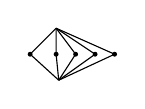
\begin{tikzpicture}[scale=.33,baseline=0pt]\coordinate (a) at (0,1);\coordinate (b) at (.1,-1);\foreach \x in {-1,0,.75,1.5,2.25}{\draw (a)--(\x,0)--(b);\fill (\x,0) circle(2.7pt);}\end{tikzpicture}}\\=\text{fausse 5-base}} & \mathrm{Ens}_5\times\mathrm{Ens}_2 & \substack{\text{cf plus haut}\\2^\circ} & 15 & \substack{1,1,5,\\5,5,10}\\ \hline
 & \text{triade }\deleted{\unsure{\text{triang}}}\inserted{\text{ordonnée}} & \substack{\inserted{\mathrm{Ens}_3\times\mathrm{Ens}_3\times\mathrm{Ens}_3}\\\deleted{\unsure{\mathfrak S_3\times\mathfrak S_3\times\mathfrak S_3}}} & \substack{\mathfrak S_3\times\mathfrak S_3\times\mathfrak S_3\\\text{ordre }6^3=2^3.3^3=216} & 2^4.3.5=240 & 9,9,9\\ \hline
 & \text{triades}\quad /\!/\!/ & \substack{\unsure{\text{puiss.}|\text{perm.}}\text{ d'ordre }3\\\text{d'un ens card. }3\simeq\\\text{ens de card. }9\text{ avec partition}} & \substack{\mathfrak S_3.(\mathfrak S_3\times\mathfrak S_3\times\mathfrak S_3)\\\text{card }6^4=2^4 3^4} & 2^3.5=40 & 27\\ \hline
 & \text{grilles 3-carrée}\unsure{\text{s}} & \substack{\text{comme dessus, avec}\\\text{une partie distinguée}} & \mathfrak S_2.(\mathfrak S_3\,\mathfrak S_3\,\mathfrak S_3) & 2^3.3.5=120 & 9,18\\ \hline
 & \substack{\text{arête}\quad\text{---}\\\simeq\text{triangle pointé}} &  &  &  & \\ \hline
 & \substack{\text{arcs}\quad\longrightarrow\\\sim\text{ triangle ordonné}} &  &  &  & \\ \hline
 & \text{triangles }\triangle &  &  &  & \\ \hline
 & \text{
\begin{tikzpicture}[baseline=0pt,scale=.35]\draw (-.6,.8)--(0,-.35)--(.6,.8);\foreach \x/\y in {-.6/.8,0/-.35,.6/.8}{\fill (\x,\y) circle(3pt);}\end{tikzpicture}} &  &  &  & \\ \hline
\unsure{\frac{120}{16}|13^\circ,\ 16} & \left(\text{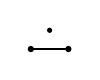
\begin{tikzpicture}[baseline=0pt,scale=.34]\draw (0,0)--(1.4,0);\fill (0,0) circle(3.4pt);\fill (1.4,0) circle(3.4pt);\fill (.7,.7) circle(2.8pt);\end{tikzpicture}}\right)\simeq(\text{arcs}) &  &  &  & 
\end{array}$}}
% archive sheet number: 61

\scanpage{63}
% letterhead
\begin{tabular}{c}
UNIVERSITE DES SCIENCES ET TECHNIQUES\\
DU LANGUEDOC\\
---\\
INSTITUT DE MATHEMATIQUES\\
Place Eugène Bataillon\\
34060 MONTPELLIER CEDEX
\end{tabular}
\hfill Montpellier, le

\[
\begin{aligned}
&\deleted{(r_1+r_{i-1})+}\\
&(r_1\ldots+r_{i-1})+(r_2\ldots+r_{j-1})+(r_3+\ldots+r_{k-1})\\
&i\ge3 \qquad\qquad\qquad\unsure{{}+r_1}\\
&r_1+2(r_2\ldots+r_{i-1})
\end{aligned}
\]
\[
\begin{aligned}
&\delta_1\ -\ \delta_8\,\underline{\delta_9}
&&r_1&&r_1+2r_2&&i-1&&i{}+j+\unsure{h|k}-6\\
&\delta_1\ -\ \underline{\delta_n}\,\delta_{n+1}
&&r_1+r_2+r_3&& &&j-2\\
&n+1+9\le27&&r_2+r_3+r_4&& &&k-3\\
&n\le17&&r_3+r_4+r_5
\end{aligned}
\]
\figure{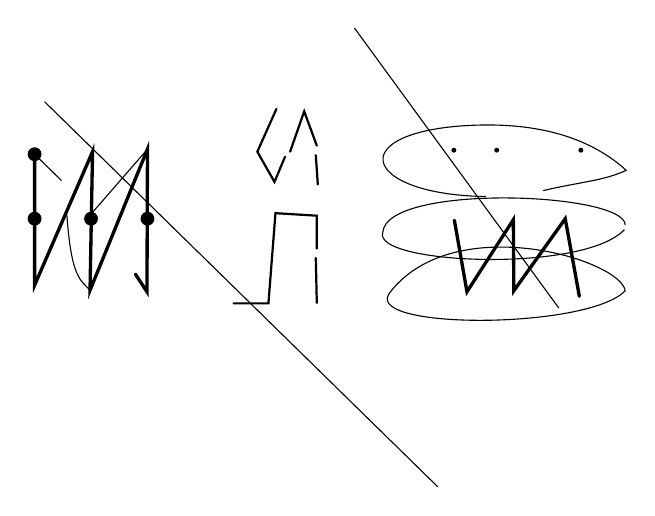
\begin{tikzpicture}[x=.64cm,y=.64cm,line cap=round]
\draw[very thick] (0,2.6)--(0,0)--(1.15,2.65)--(1.1,-.1)--(2.24,2.7)--(2.23,-.13)--(2.0,.22);
\draw (0,2.6)--(.53,2.08) (.64,1.4) .. controls (.73,.14) and (.91,.11) .. (1.1,-.1) (1.11,1.4)--(2.24,2.7);
\foreach \x in {0,1.12,2.24}{\fill (\x,1.32) circle(2.5pt);}
\fill (0,2.6) circle(2.5pt);
\draw[thick] (4.8,3.5)--(4.42,2.65)--(4.76,2.05)--(4.97,2.55) (5.07,2.65)--(5.35,3.45)--(5.6,2.77) (5.58,2.58)--(5.62,2.0);
\draw[thick] (3.95,-.36)--(4.64,-.36)--(4.78,1.43)--(5.60,1.38)--(5.6,.73) (5.58,.54)--(5.60,-.35);
\draw (8.95,1.76) .. controls (6.55,1.8) and (6.13,2.98) .. (8.45,3.16) .. controls (10.24,3.29) and (11.2,2.77) .. (11.74,2.28) .. controls (11.28,2.07) and (10.88,2.06) .. (10.1,1.88);
\draw (11.72,1.20) .. controls (11.69,1.85) and (6.98,2.02) .. (6.91,1.05) .. controls (6.68,.42) and (10.88,.23) .. (11.70,1.1);
\draw (11.72,-.11) .. controls (11.63,.51) and (8.35,1.49) .. (7.07,-.12) .. controls (6.37,-.89) and (10.97,-.89) .. (11.72,-.11);
\foreach \x in {8.32,9.17,10.84}{\fill (\x,2.68) circle(.9pt);}
\draw[very thick] (8.33,1.29)--(8.58,-.13)--(9.5,1.3)--(9.51,-.11)--(10.53,1.32)--(10.81,-.22);
\draw[thin] (.2,3.64)--(8,-4.0) (6.35,5.1)--(10.4,-.45);
\end{tikzpicture}}

% Lower part read with the sheet rotated through 180 degrees.
\[
\begin{aligned}
r_0&=2\eta-\zeta\\
r_1&=\zeta_1-\zeta_2\\
r_2&=\zeta_2-\zeta_3\\
r_3&=\zeta_3-\zeta_4\\
r_4&=\zeta_4-\zeta_5\ .\\
r_5&=\zeta_5-\zeta_6\\
\deleted{\unsure{r_6}}&=\\
r_6&=\eta-\zeta_1-\zeta_2-\zeta_3
\end{aligned}
\qquad
\left.\begin{aligned}
3(r_1+r_2+r_3)&=3(\zeta_1-\zeta_4)\\
2r_4&=\deleted{\unsure{3}}\zeta_4\deleted{\unsure{+}}-2\zeta_5\\
\unsure{2}r_5&=\deleted{\unsure{2}}\zeta_5-\zeta_6
\end{aligned}\right\}\quad3\zeta_1-\zeta_4-\zeta_5-\zeta_6
\]
\figure{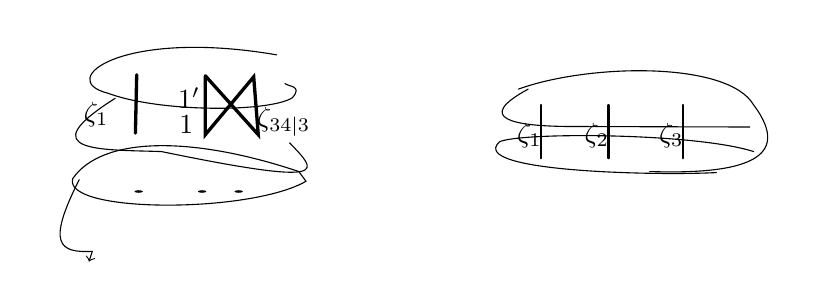
\begin{tikzpicture}[x=.83cm,y=.65cm,line cap=round]
\draw (2.8,2.7) .. controls (.43,3.22) and (-.6,2.21) .. (.22,1.95) .. controls (.99,1.58) and (2.67,1.57) .. (3.04,1.86) .. controls (3.21,2.1) and (2.97,2.08) .. (2.93,2.14);
\draw (.33,1.85) .. controls (-1.0,.78) and (.15,.85) .. (1.04,.81) .. controls (3.7,.11) and (3.42,.42) .. (3.0,.98);
\draw (3.14,.42) .. controls (1.48,1.13) and (.12,1.1) .. (-.32,.28) .. controls (-.47,-.4) and (2.40,-.4) .. (3.25,.23) --(3.14,.42);
\foreach \x in {.69,1.66,2.22}{\fill (\x,.03) ellipse(.065 and .025);}
\draw[very thick] (.66,2.31)--(.64,1.17) (1.71,2.29)--(1.71,1.14)--(2.45,2.27)--(2.52,1.14)--(1.71,2.29);
\node at (.04,1.53) {$\zeta_1$};\node at (1.46,1.85) {$\unsure{1'}$};\node at (1.42,1.33) {$\unsure{1}$};\node at (2.91,1.40) {$\zeta_{\unsure{34|3}}$};
\draw[->] (-.22,.26) .. controls (-.72,-1) and (-.53,-1.17) .. (-.02,-1.14)--(-.07,-1.34);
\draw (6.5,2.03) .. controls (7.58,2.53) and (9.71,2.58) .. (10.1,1.72) .. controls (10.72,.66) and (9.94,.36) .. (8.51,.42);
\draw (6.65,2.03) .. controls (5.81,1.45) and (6.43,1.31) .. (7.26,1.3)--(10.04,1.29);
\draw (10.10,.81) .. controls (9.2,1.18) and (6.51,1.19) .. (6.21,1.0) .. controls (5.70,.40) and (8.71,.34) .. (9.53,.40);
\foreach \x/\y in {6.85/1,7.88/2,9.02/3}{\draw[thick](\x,.68)--(\x,1.72);\node at (\x-.18,1.12) {$\zeta_{\y}$};}
\end{tikzpicture}}
% archive sheet number: 62

\scanpage{64}
\[
\begin{aligned}
r_0&=2\eta-\zeta\\
r_{ij}&=\zeta_i-\zeta_j\qquad i<j\\
r_{\{i,j,h\}}&=\deleted{\left(\begin{smallmatrix}\zeta_i,\zeta_j,\zeta_h,\zeta_{mn},\zeta_{n\ell},\zeta_{\ell m}\\
\zeta_{jh},\zeta_{hi},\zeta_{ij},\zeta'_\ell,\zeta'_m,\zeta'_n\end{smallmatrix}\right)}
=\zeta_{jh}-\zeta_i=\zeta_{hi}-\zeta_j=\zeta_{ij}-\zeta_h\\
&=\zeta'_\ell-\zeta_{mn}=\zeta'_m-\zeta_{n\ell}=\zeta'_n-\zeta_{\ell m}\\
&=\eta-\zeta_i-\zeta_j-\zeta_h
\end{aligned}
\]
\[
\begin{gathered}
\left(\begin{matrix}\zeta_1&-&\zeta_6\\\zeta'_1&-&\zeta'_6\end{matrix}\right)\\
\begin{matrix}(\zeta_j,\zeta'_j,\zeta_{i\ell}&\ell\ne i,j)\\\zeta_i,\zeta'_i,\zeta_{j\ell}&\ell\ne i,j\end{matrix}\\
\left(\begin{matrix}\zeta_i,\zeta_j,\zeta_h,&\zeta_{mn},\zeta_{n\ell},\zeta_{\ell m}\\
\zeta_{jh},\zeta_{hi},\zeta_{ij},&\zeta'_\ell,\zeta'_m,\zeta'_n\end{matrix}\right)
\end{gathered}
\]
% margin note written sideways
\margin{$\begin{smallmatrix}&&&\zeta'_1&\zeta'_2&\zeta_{24}&\zeta_{56}&(\unsure{\zeta'})\\
\zeta_1&\zeta'_2&\zeta_3&\lambda_{34}&\deleted{\unsure{\zeta'_{56}}}&56&\deleted{\unsure{\zeta_1,\zeta_2}}\end{smallmatrix}$\quad
$\unsure{\zeta_1}\ \zeta_{12}\ \zeta'_1\ \zeta_{\unsure{3|8}}$}
\figure{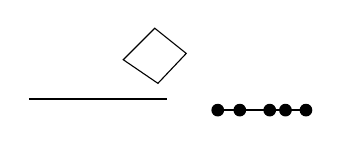
\begin{tikzpicture}[x=.4cm,y=.4cm]\draw (0,0)--(1,1)--(2,.2)--(1.1,-.75)--cycle;
\draw[thick](-3,-1.25)--(1.4,-1.25);
\draw[thick](3,-1.6)--(3.7,-1.6) (3.9,-1.6)--(5.8,-1.6);
\foreach \x in {3,3.7,4.65,5.15,5.8}{\fill(\x,-1.6) circle(2.3pt);}\end{tikzpicture}}
\diagram{\begin{tikzcd}[ampersand replacement=\&,column sep=tiny,row sep=small]
\& r_{456}\arrow[dr,dash]\arrow[rr,dashed,dash]\&\&r_0\arrow[dl,dash]\arrow[dr,dashed,dash]\&\\
-r_{1,2,3}=-r_6\arrow[rr,dash]\&\&{}\arrow[rr,dash]\arrow[dl,dash]\arrow[dr,dash]\&\&r_{123}=r_6\\
\&-r_0\&\&-r_{4,5,6}\&
\end{tikzcd}}
\[
\frac{-\langle r,r'\rangle}{\sqrt{\langle r,r\rangle\langle r',r'\rangle}}=\frac{\langle r,r'\rangle}{-2}
\]
\[
\begin{aligned}
r_{\unsure{0}}r_{ij}&=0\\
r_0\,r_{ijh}&=-1\\
r_{ij}\,r_{i',j'}&=\begin{cases}
0&\text{si }\{i,j\}\cap\{i',j'\}=\varnothing\\
\pm1&\text{si }\{i,j\}\cap\{i',j'\}\ne\varnothing
\end{cases}
\quad\begin{aligned}
+1&\quad\text{si }\deleted{i<j\le i'<j'\ \text{ou}\ i'<j'=i<j}\ \inserted{i'=j\ \text{ou}\ i=j'}\\
-1&\quad\text{si }i\ne i'\ \text{ou}\ j=j'
\end{aligned}\\
r_{ijh}.r_{pqr}&=1-\operatorname{card}(\{i,j,h\}\cap\{p,q,r\})=
\begin{cases}-1&\text{si }\operatorname{card}\{i,j,h\}\cap\{i',j',h'\}=2\\
0&\text{si }\rule{6em}{.3pt}=1\\1&\text{si }\rule{6em}{.3pt}=0\end{cases}\\
r_{ij}\,r_{p,q,r}&=\begin{cases}
0&\text{si }\{i,j\}\unsure{\subset|\in}\{p,q,r\}\text{ ou }\{i,j\}\cap\{p,q,r\}=\varnothing\\
\pm1&\text{si }\operatorname{card}\{i,j\}\cap\{p,q,r\}=1
\end{cases}\quad
\begin{cases}+1&\text{si }i\in\{p,q,r\}\\-1&\text{si }j\in\{p,q,r\}\end{cases}
\end{aligned}
\]
\[
\begin{aligned}
\zeta_1\,\zeta_2\,\zeta_3\quad\zeta_4,\zeta_5\,\zeta_6&=r_0=2\eta-\zeta
= \quad=3(r_1+r_2+r_3)+2r_4+r_5+2r_6\\
\zeta_1\,\zeta_2\,\zeta_3\quad\zeta'_{56}\,\zeta_{64}\,\zeta_{45}
&=r_{123}=\eta-\zeta_1-\zeta_2-\zeta_3=r_6\\
\zeta_{\unsure{23}}\,\zeta_{31},\zeta_{12}\quad\zeta_4\,\zeta_5\,\zeta_6
&=r_{4,5,6}=\eta-\zeta_4-\zeta_5-\zeta_6=r_6+3(r_1+r_2+r_3)+2r_4+r_5 .
\end{aligned}
\]
\diagram{\begin{tikzcd}[ampersand replacement=\&,column sep=tiny,row sep=tiny]
\&r_{\unsure{4}56}\arrow[rr,dash]\&\&r_{\unsure{0}}\deleted{\unsure{6}}\arrow[dr,dash]\&\\
-r_{\unsure{6|65}}\&\&{}\arrow[ul]\arrow[ur,Rightarrow]\arrow[ll,dash]\arrow[rr,dash]\arrow[dl,Rightarrow]\arrow[dr,dash]\&\&r_{\unsure{6|034}}\\
\&-r_{\unsure{0|023}}\&\&-r_{4,56}\&
\end{tikzcd}}
% archive sheet number: 63

\scanpage{67}
\uline{Parties $i$-libres} etc

On étudie des types de diagrammes plongés dans les complexes cubiques $C$, liés directement aux parties $n$-libres \deleted{\unsure{ou $n$-bases}} (parties de cardinal $n$ de $C$ formées de sommets non liés deux à deux). Signalons \deleted{tout} de suite

\uline{Prop} \textcircled{1} Pour qu'il existe dans $C$ une partie $n$-libre, \deleted{\unsure{il}} faut s. que $1\leq n\leq6$. Les parties $n$-libres maximales \inserted{s}/sont : \deleted{celles}

a) celles de cardinal $6$, ce sont aussi des bases

b) \deleted{celles de cardinal $5$ qui sont \unsure{représentées}} \inserted{les parties} de la \deleted{forme} $E(x)\cap E(y)$, où $x,y$ sont deux sommets distincts \unsure{non liés|deux liés} de $C$. Ce sont des parties de cardinal $5$.

\textcircled{2} Soit $L_{\unsure{n|i}}$ \quad $1\leq\deleted{\unsure{n}}i\leq6$ le graphe discret \inserted{$[1,i]$} de cardinal $i$ (pas de liens). Alors \deleted{pour} $i\ne5$, l'ens $\mathrm{Pl}(L_n,C)$ des plongements de $L_n$ dans $C$ est un espace homogène sous $W=\mathrm{Aut}(C)$. Pour $i=5$, il a deux orbites \inserted{$\mathrm{Pl}(L_5,C)'$ et $\mathrm{Pl}(L_5,C)''$} pour $W$, savoir

a) les $5$-bases, i.e. parties $5$-libres qui sont contenues dans une base -- une !

b) les demi étoiles, i.e. parties de la forme $E(x)\cap E(y)$, où $x,y$ sont deux sommets distincts non liés

Les applications \deleted{Pl} (hom d'un pas en bas)

\diagram{\resizebox{\linewidth}{!}{$\begin{tikzcd}[ampersand replacement=\&,column sep=small,row sep=small]
{} \& {} \& {} \& {} \& {} \& \mathrm{Pl}''(L_5,C)\arrow[dl,"1"'] \& {}\\
\underset{\substack{\Vert\\\mathrm{Pl}(L_0,C)}}{\mathrm{pt}} \& \underset{\substack{\Vert\\D_1}}{\mathrm{Pl}(L_1,C)}\arrow[l,"27"'] \& \mathrm{Pl}(L_2,C)\arrow[l,"16"'] \& \mathrm{Pl}(L_3,C)\arrow[l,"10"'] \& \mathrm{Pl}(L_4,C)\arrow[l,"6"'] \& \mathrm{Pl}'(L_5,C)\arrow[l,"2"'] \& \mathrm{Pl}(L_6,C)\arrow[l,"1"']
\end{tikzcd}$}}

sont surjectives, et les degrés de projection sont \deleted{respectivement} \deleted{$27,16,\unsure{90|10},6$} ceux marqués (cf \unsure{dévissage|dénissage|dessin} plus bas), d'où on tire les cardinaux des $i$-bases \unsure{épinglées}

% archive sheet number: 66
